\documentclass[12pt]{article}
\usepackage[a4paper]{geometry}
\usepackage{fullpage}
\usepackage[T1]{fontenc}
\usepackage[utf8]{inputenc}
\usepackage{graphicx}
\usepackage{mathpazo}
\pagenumbering{gobble}
\usepackage{siunitx}
\sisetup{output-decimal-marker = {,}}
\usepackage{amsmath}
\usepackage{esdiff}
\usepackage[spanish]{babel}
\usepackage{steinmetz}
\usepackage{pdfpages}

\begin{document}

\title{\textsc{Teoría de Circuitos II} :: Acoplamientos}

\date{}

\maketitle
En el circuito de la figura:
\begin{enumerate}
\item Escribe las ecuaciones de mallas sin realizar la sustitución numérica.
\item Tras realizar la sustitución numérica, resuelve las ecuaciones anteriores, y obtén las corrientes de rama indicadas.
\item Realiza un balance de potencias activas.
\end{enumerate}

\begin{center}
  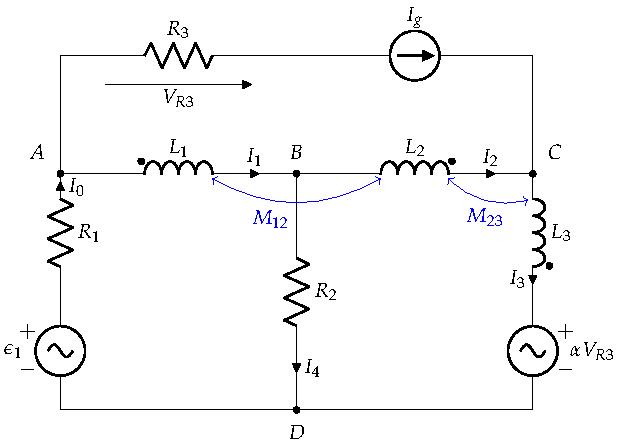
\includegraphics[height=0.4\textheight]{figs/acoplamientos.pdf}
\end{center}

Datos:

\begin{align*}
  \overline{I}_g &= \SI[parse-numbers=false]{10\phase{\ang{0}}}{\ampere}\\
  \overline{\epsilon}_1 &= \SI[parse-numbers=false]{10\phase{\ang{0}}}{\ampere}\\
  R_i &= \SI{1}{\ohm} \quad \forall i\\
  X_{Li} &= \SI{1}{\ohm} \quad \forall i\\
  \alpha &= 1\\
\end{align*}

Todos los acoplamientos magnéticos del circuito son perfectos.

\subsection*{Solución}
Tomando las tres corrientes de malla en sentido dextrógiro, siendo $I_a$ la corriente de la malla inferior izquierda, $I_b$ la corriente de la malla inferior derecha, e $I_c$ la corriente de la malla superior, las ecuaciones de las dos mallas inferiores son:
\begin{align*}
  \overline{\epsilon}_1 &= \overline{I}_a (R_1 + j \omega L_1 + R_2) + \\
                        &+ \overline{I}_b (-R_2 - j \omega M_{12}) +\\
                        &+ \overline{I}_c (-j \omega L_1 + j \omega M_{12})
\end{align*}

\begin{align*}
  - \alpha \overline{U}_{R3} &= \overline{I}_a (-R_2 - j \omega M_{12}) + \\
                        &+ \overline{I}_b (R_2 + j\omega L_2 + j\omega L_3 + 2j\omega M_{23}) +\\
                        &+ \overline{I}_c (-j \omega L_2 - j \omega M_{23} + j\omega M_{12})
\end{align*}

Además,

\begin{align*}
  \overline{I}_c &= \overline{I}_g\\
  \overline{U}_{R3} &= R_3 \overline{I}_g
\end{align*}

Reagrupando obtenemos:
\begin{align*}
  \overline{\epsilon}_1 + \overline{I}_g (j \omega L_1 - j \omega M_{12}) &= \overline{I}_a (R_1 + j \omega L_1 + R_2) + \overline{I}_b (-R_2 - j \omega M_{12})\\
  \overline{I}_g (j \omega L_2 + j \omega M_{23} - j\omega M_{12} - \alpha R_3) &= \overline{I}_a (-R_2 - j \omega M_{12}) + \overline{I}_b (R_2 + j\omega L_2 + j\omega L_3 + 2j\omega M_{23})
\end{align*}

Realizamos la sustitución numérica, 

\begin{align*}
  10 &= \overline{I}_a (2 + j) + \overline{I}_b (-1 - j)\\
  10 (-1 + j) &= \overline{I}_a (-1 - j) + \overline{I}_b (1 + 4j)
\end{align*}

donde se ha tenido en cuenta que:

\begin{align*}
  \omega M_{12} &= \sqrt{\omega L_1 \cdot \omega L_2} = \SI{1}{\ohm}\\
  \omega M_{23} &= \sqrt{\omega L_2 \cdot \omega L_3} = \SI{1}{\ohm}
\end{align*}
La solución de este sistema es:

\begin{align*}
  \overline{I}_a &= \SI[parse-numbers=false]{5.66\phase{\ang{-1.91}}}{\ampere} = \SI[parse-numbers=false]{5.66 - 0.19j}{\ampere}\\
    \overline{I}_b &= \SI[parse-numbers=false]{3.88\phase{\ang{29.05}}}{\ampere} = \SI[parse-numbers=false]{3.39 + 1.89j}{\ampere}
\end{align*}

Las corrientes de rama indicadas son:

\begin{align*}
  \overline{I}_0 &= \SI[parse-numbers=false]{5.66 - 0.19j}{\ampere}\\
  \overline{I}_1 &= \SI[parse-numbers=false]{-4.33 - 0.19j}{\ampere}\\
  \overline{I}_2 &= \SI[parse-numbers=false]{-6.6 + 1.88j}{\ampere}\\
  \overline{I}_3 &= \SI[parse-numbers=false]{3.39 + 1.88j}{\ampere}\\
  \overline{I}_4 &= \SI[parse-numbers=false]{2.26 - 2.07j}{\ampere}
\end{align*}

Finalmente, las potencias activas de los generadores son:

\begin{align*}
  P_{\epsilon1} &= Re(\overline{\epsilon}_1 \cdot \overline{I}_0^*) = \SI{56.6}{\watt}\\
  P_{\alpha} &= Re(\alpha R_3 \overline{I}_g \cdot (-\overline{I}_3)^*) = \SI{-33.96}{\watt}\\
  P_{\epsilon1} &= Re(\overline{U}_{Ig} \cdot \overline{I}_g^*) = \SI{118.87}{\watt}
\end{align*}
donde la tensión $U_{Ig}$ se calcula con:

\begin{align*}
  \overline{U}_{AC} &= \overline{U}_{R3} - \overline{U}_{Ig}\\
  \overline{U}_{AC} &= \overline{U}_{L1} + \overline{U}_{L2}\\
  \overline{U}_{L1} &= \overline{I}_1 j \omega L_1 - \overline{I}_2 j \omega M_{12}\\
  \overline{U}_{L2} &= - \overline{I}_1 j \omega M_{12} + \overline{I}_2 j \omega L_2 + \overline{I}_3 j \omega M_{23}
\end{align*}
  
Las potencias de las resistencias son:

\begin{align*}
  P_{R1} &= R_1 I_0^2 = \SI{32.08}{\watt}\\ 
  P_{R2} &= R_2 I_4^2 = \SI{9.43}{\watt}\\ 
  P_{R3} &= R_3 I_g^2 = \SI{100}{\watt}
\end{align*}

Comprobamos que la potencia activa total entregada por las fuentes coincide con la potencia activa total consumida en las resistencias.
\end{document}

% Local Variables:
% ispell-local-dictionary: "castellano"
% End:

